\def\year{2021}\relax

\documentclass[letterpaper]{article} % DO NOT CHANGE THIS
\usepackage{aaai21}  % DO NOT CHANGE THIS
\usepackage{times}  % DO NOT CHANGE THIS
\usepackage{helvet} % DO NOT CHANGE THIS
\usepackage{courier}  % DO NOT CHANGE THIS
\usepackage[hyphens]{url}  % DO NOT CHANGE THIS
\usepackage{graphicx} % DO NOT CHANGE THIS
\urlstyle{rm} % DO NOT CHANGE THIS
\def\UrlFont{\rm}  % DO NOT CHANGE THIS
\usepackage{natbib}  % DO NOT CHANGE THIS AND DO NOT ADD ANY OPTIONS TO IT
\usepackage{caption} % DO NOT CHANGE THIS AND DO NOT ADD ANY OPTIONS TO IT
\frenchspacing  % DO NOT CHANGE THIS
\setlength{\pdfpagewidth}{8.5in}  % DO NOT CHANGE THIS
\setlength{\pdfpageheight}{11in}  % DO NOT CHANGE THIS
%\nocopyright
%PDF Info Is REQUIRED.
% For /Author, add all authors within the parentheses, separated by commas. No accents or commands.
% For /Title, add Title in Mixed Case. No accents or commands. Retain the parentheses.
\pdfinfo{
/Title (Analysis of Olympic Tweets from Tokyo 2020)
/Author (Naman Bhargava, Jordan Rodrigues)
/TemplateVersion (2021.2)
} %Leave this
% /Title ()
% Put your actual complete title (no codes, scripts, shortcuts, or LaTeX commands) within the parentheses in mixed case
% Leave the space between \Title and the beginning parenthesis alone
% /Author ()
% Put your actual complete list of authors (no codes, scripts, shortcuts, or LaTeX commands) within the parentheses in mixed case.
% Each author should be only by a comma. If the name contains accents, remove them. If there are any LaTeX commands,
% remove them.

% DISALLOWED PACKAGES
% \usepackage{authblk} -- This package is specifically forbidden
% \usepackage{balance} -- This package is specifically forbidden
% \usepackage{color (if used in text)
% \usepackage{CJK} -- This package is specifically forbidden
% \usepackage{float} -- This package is specifically forbidden
% \usepackage{flushend} -- This package is specifically forbidden
% \usepackage{fontenc} -- This package is specifically forbidden
% \usepackage{fullpage} -- This package is specifically forbidden
% \usepackage{geometry} -- This package is specifically forbidden
% \usepackage{grffile} -- This package is specifically forbidden
% \usepackage{hyperref} -- This package is specifically forbidden
% \usepackage{navigator} -- This package is specifically forbidden
% (or any other package that embeds links such as navigator or hyperref)
% \indentfirst} -- This package is specifically forbidden
% \layout} -- This package is specifically forbidden
% \multicol} -- This package is specifically forbidden
% \nameref} -- This package is specifically forbidden
% \usepackage{savetrees} -- This package is specifically forbidden
% \usepackage{setspace} -- This package is specifically forbidden
% \usepackage{stfloats} -- This package is specifically forbidden
% \usepackage{tabu} -- This package is specifically forbidden
% \usepackage{titlesec} -- This package is specifically forbidden
% \usepackage{tocbibind} -- This package is specifically forbidden
% \usepackage{ulem} -- This package is specifically forbidden
% \usepackage{wrapfig} -- This package is specifically forbidden
% DISALLOWED COMMANDS
% \nocopyright -- Your paper will not be published if you use this command
% \addtolength -- This command may not be used
% \balance -- This command may not be used
% \baselinestretch -- Your paper will not be published if you use this command
% \clearpage -- No page breaks of any kind may be used for the final version of your paper
% \columnsep -- This command may not be used
% \newpage -- No page breaks of any kind may be used for the final version of your paper
% \pagebreak -- No page breaks of any kind may be used for the final version of your paperr
% \pagestyle -- This command may not be used
% \tiny -- This is not an acceptable font size.
% \vspace{- -- No negative value may be used in proximity of a caption, figure, table, section, subsection, subsubsection, or reference
% \vskip{- -- No negative value may be used to alter spacing above or below a caption, figure, table, section, subsection, subsubsection, or reference

\setcounter{secnumdepth}{0} %May be changed to 1 or 2 if section numbers are desired.

% The file aaai21.sty is the style file for AAAI Press
% proceedings, working notes, and technical reports.
%

% Title

% Your title must be in mixed case, not sentence case.
% That means all verbs (including short verbs like be, is, using,and go),
% nouns, adverbs, adjectives should be capitalized, including both words in hyphenated terms, while
% articles, conjunctions, and prepositions are lower case unless they
% directly follow a colon or long dash


\title{Analysis of Olympic Tweets from Tokyo 2020}
\author{
    %Authors
    % All authors must be in the same font size and format.
    Naman Bhargava, Jordan Rodrigues\\
}
\affiliations{
    %Afiliations
    Georgia Institute of Technology\\
    %If you have multiple authors and multiple affiliations
    % use superscripts in text and roman font to identify them.
    %For example,

    % Sunil Issar, \textsuperscript{\rm 2}
    % J. Scott Penberthy, \textsuperscript{\rm 3}
    % George Ferguson,\textsuperscript{\rm 4}
    % Hans Guesgen, \textsuperscript{\rm 5}.
    % Note that the comma should be placed BEFORE the superscript for optimum readability

    North Ave NW\\
    Atlanta, GA 30332\\
    nbhargava9@gatech.edu, jrodrigues30@gatech.edu
    % email address must be in roman text type, not monospace or sans serif
    %publications21@aaai.org

    % See more examples next
}


\begin{document}

\maketitle

\begin{abstract}
    This work seeks to understand how and why individuals utilized Twitter to engage with the 2020 Tokyo Olympics via tweet data with the hashtag \emph{\#Tokyo2020} from [start date] to [end date]. We  extend on previous work that analyzed the 2010, 2012, and 2016 Olympics, as well as studies on Twitter engagement for the NBA and the 2014 World Cup. In particular, we aim to answer [rq1], [rq2], and [rq3] through the usage of [tech1], [tech2], and [tech3]
    %Briefly summarize the goal, related work, research goals/questions, and methods of the research project.
\end{abstract}

\section{Introduction}

The Olympic Games are one of the world's most universal athletic competitions, drawing more than 200 competing nations [\#1]. Digital engagement with the Olympics has also been increasing drastically, with more than 100 million unique users participating for Tokyo 2020, doubling the amount of users from the previous Summer Olympics [\#2]. Of the online platforms, Twitter captured a majority share of Olympics discussion, generating more than 75 billion impressions during Rio 2016 (compared to Facebook's 1.5 billion interactions) [\#3]. As online engagement has increased, so too has the diversity of discussion that takes places during the event; individuals converse about the introduction of new sports, the performance of athletes, and celebrate the success of their nations. However, not all Twitter discussion is positive. Following the emergence of COVID-19, anti-asian racism and xenophobia rose drastically [\#4], prompting significant controversial discussion around the postponement of Tokyo 2020, as well as COVID protocols for the games. Negative sentiment is also often displayed against competing nations and individual athletes as well.

We seek to conduct a holistic overview of Twitter discussion during the Tokyo 2020 Olympics. This will include studying [rq1], [rq2], and [rq3]. These questions will be answered via the \emph{Tokyo 2020 Olympics Tweets Dataset} [\#5], which contains a sample of tweets using the hashtag \emph{\#Tokyo2020} between 07/24/2021 and 07/27/2021, the beginning of the Games.

What is the motivating problem for your research project? What are the research questions to be examined for the project? If you are contributing a dataset, what do you envision the output of your work to look like? Who can use this dataset, and on what kind of problems would this dataset be ideal? If you are contributing analysis, how are these findings theoretically significant or broadly important for society?
-0.5 pts, introduction does not clearly describe a motivating problem
-1 pt, introduction does not mention the research goals/questions clearly

\section{Related Work}
Other works have looked at Olympics related discussions through tweets on Twitter. Sentiment analysis was conducted on a Rio de Janeiro Olympic tweets dataset released by \cite{VERTALKA2019103869}. This dataset included over 21 million tweets with location data, language, and tweet content. This sentiment analysis was done in \cite{KASSENSNOOR2019229}, finding tweets about host cities were positive, while tweets about the IOC were negative. The study scored tweet sentiment by taking the difference between positive and negative key words matched from the Mohammad and Turney's (2010) lexicon. This method meant only English language tweets could be scored. This work was important to show the positive effects on host city image perception from hosting the Olympics on a global population. Our work focuses more on understanding different topics and sentiments around those topics of discussion, rather than just focussing on host cities. 

General sentiment analysis and engagement is explored by \cite{5718715} during the Winter 2010 Olympics. This paper found positive tweets were forwarded more, and that negative users were more passionate. The study calculated sentiment using the SentiStrength system. The work poses future questions on how people engage or cluster around topics or tweet tones, and how social network impacts engagement. Our work focuses on understanding the topics that have the highest engagement. 


\section{Methods}
For our data we will be working with two \emph{Tokyo 2020 Olympics Tweet} Datasets [#5, #6] on Kaggle. The first dataset queries a sample of tweets with the hashtag \emph{#Tokyo2020} between 07/24/2021 - 07/27/2021, leading to a total of 160K+ tweets. The second dataset was run daily from 07/25/2021 - 07/31/2021. We'll use distinct tweet_ids to filter duplicate tweets. Both of these datasets share common features such as user location, tweet content, info on retweets and favorites, as well as info on user popularity (measured by friend and follower count). 

Our research questions are as follows. 1) How does Twitter discussion around the Olympics vary as a function of region/location? We want to better understand whether regions have differences in the prevailing sentiment when they discuss the Olympics as well as whether there are differences in the types of Olympic-related topics that are discussed.

2) What are the most common themes/topics that emerged during the discussion of the Tokyo 2020 Olympics? Abstracting away the regional component, we want to understand the 'Twitter scene' as a whole. Were Twitters users mainly focused on discussing the events themselves, athletes, COVID-19, or other Olympics-related controversies?

3) How do tweet characteristics impact tweet virulence? Is there a relationship between tweet sentiment and virulence (defined as a linear combination of likes and retweets)? What about topics and virulence? Do we find that a small portion of users drive a large proportion of virulent Olympics tweets; if so, what are the characteristics of these users?

To answer our research questions, we start by completing an initial cleaning of the data. This will by filtering out incoherent tweets (empty spaces, random characters) as well as eliminating non-English tweets. While we note that this can potentially lead to inaccurate representations of regional trends (as English-tweeting individuals may not be representative of all tweeters in other regions), language-aware modeling will be left to future work. We then intend to carry out other elements of text processing such as stopword removal, stemming, and lemmatization. 

These 'processed' texts will allow us to perform topic modeling, which will be carried out the Gensim implementation of Latent Dirichlet Allocation (LDA). These topics will then drive insights around thematic emergence both regionally and non-regionally. We can then statistically test to see if topics vary on a geographic basis by aggregating the topic distributions produced our LDA model on a regional basis (via average) and running a Kolmogorov-Smirnov test. For example, we may average the topic distributions for each Brazilian Tweet and each United States Tweet separately to see if there is a statistically significant difference it what the regions discuss.

Finally, to study how tweet characteristics impact tweet virulence for Olympic discussion, we plan on carrying out a statistical analysis. We'll start by carrying out a graphical normality test (such as a QQ plot) to determine whether tweet virulence follows a normal distribution (though we suspect it does not). From here, we'll carry out ANOVA/Kruskal Wallis Tests or a T-Test/Mann-Whitney U-Test based on what dimensions of the tweets we are comparing for virulence. For example, a regional analysis may make use of Kruskal Wallis, while testing how the presence of the word 'Olympics' impacts virulence would require a Mann-Whitney. 

#consider normalizing for follower and friend counts

Methods (3 pts)
1-3 paragraphs explaining your research methodology. What data will you use? What model? What statistical tests will you run?
-1.5 pt, the data pipeline is not clearly or specifically described 
-1.5 pt, the computational model / statistical analysis is not clearly or specifically described 




\section{Timeline}
1 short paragraph describing a weekly timeline for your project and task responsibilities by team members. By when do you hope to have acquired your data? When will you build or select the statistical / computational models and when will you run them? When will you finalize the main analyses and plots and paper writing? 
-0.5 pts, basic project milestones are not identified and assigned to team members
-0.5 pts, rough dates for completing basic project milestones have not been identified




\subsection{Page Breaks}
For your final camera ready copy, you must not use any page break commands. References must flow directly after the text without breaks. Note that some conferences require references to be on a separate page during the review process. AAAI Press, however, does not require this condition for the final paper.


%\subsection{Overlength Papers}
%If your paper is too long and you resort to formatting tricks to make it fit, it is quite likely that it will be returned to you. %The best way to retain readability if the paper is overlength is to cut text, figures, or tables. There are, a few acceptable %ways to reduce paper size that don't affect readability. First, turn on \textbackslash frenchspacing, which will reduce the space %after periods. Next, move all your figures and tables to the top of the page. Consider removing less important portions of a %figure. If you use \textbackslash centering instead of \textbackslash begin\{center\} in your figure environment, you can also %buy some space. For mathematical environments, you may reduce fontsize {\bf but not below 6.5 point}.

%\subsection{Title and Authors}
%Your title must appear in mixed case (nouns, pronouns, and verbs are capitalized) near the top of the first page, centered over %both columns in sixteen-point bold type (twenty-four point leading). This style is called ``mixed case," which means that means %all verbs (including short verbs like be, is, using, and go), nouns, adverbs, adjectives, and pronouns should be capitalized, %(including both words in hyphenated terms), while articles, conjunctions, and prepositions are lower case unless they directly follow a colon or long dash. Author's names should appear below the title of the paper, centered in twelve-point type (with fifteen point leading), along with affiliation(s) and complete address(es) (including electronic mail address if available) in nine-point roman type (the twelve point leading). (If the title is long, or you have many authors, you may reduce the specified point sizes by up to two points.) You should begin the two-column format when you come to the abstract.







%\subsection{\LaTeX{} Copyright Notice}
%The copyright notice automatically appears if you use aaai21.sty. It has been hardcoded and may not be disabled.



%\subsection{Abstract}
%Follow the example commands in this document for creation of your abstract. The command \textbackslash begin\{abstract\} will automatically indent the text block. Please do not indent it further. {Do not include references in your abstract!}

%\subsection{Citations}
%Citations within the text should include the author's last name and year, for example (Newell 1980). Append lower-case letters to the year in cases of ambiguity. Multiple authors should be treated as follows: (Feigenbaum and Engelmore 1988) or (Ford, Hayes, and Glymour 1992). In the case of four or more authors, list only the first author, followed by et al. (Ford et al. 1997).



%\begin{quote}
%This is an example of an extract or quotation. Note the indent on both sides. Quotation marks are not necessary if you offset the text in a block like this, and properly identify and cite the quotation in the text.
%\end{quote}


\subsubsection{References.}
The references section should be labeled ``References" and should appear at the very end of the paper (don't end the paper with references, and then put a figure by itself on the last page). A sample list of references is given later on in these instructions. Please use a consistent format for references. Poorly prepared or sloppy references reflect badly on the quality of your paper and your research. Please prepare complete and accurate citations.


%IMAGE GUIDE
%\subsection{Illustrations and  Figures}
%\begin{figure}[t]
%\centering
%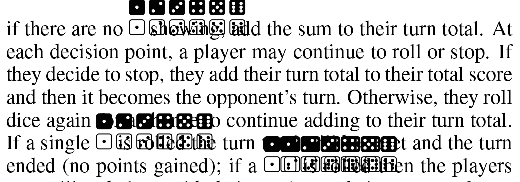
\includegraphics[width=0.9\columnwidth]{figure1} % Reduce the figure size so that it is slightly narrower than the column. Don't %use precise values for figure width.This setup will avoid overfull boxes.
%\caption{Using the trim and clip commands produces fragile layers that can result in disasters (like this one from an actual %paper) when the color space is corrected or the PDF combined with others for the final proceedings. Crop your figures properly in %a graphics program -- not in LaTeX}.
%\label{fig1}
%\end{figure}

%\begin{figure*}[t]
%\centering
%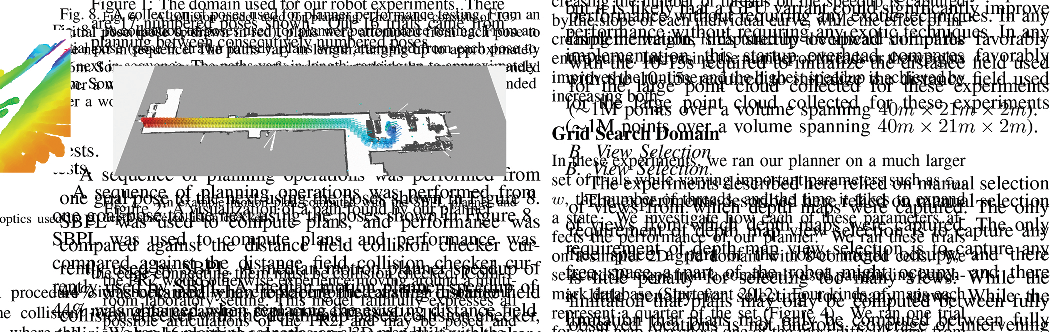
\includegraphics[width=0.8\textwidth]{figure2} % Reduce the figure size so that it is slightly narrower than the column.
%\caption{Adjusting the bounding box instead of actually removing the unwanted data resulted multiple layers in this paper. It also needlessly increased the PDF size. In this case, the size of the unwanted layer doubled the paper's size, and produced the following surprising results in final production. Crop your figures properly in a graphics program. Don't just alter the bounding box.}
%\label{fig2}
%\end{figure*}

% Using the \centering command instead of \begin{center} ... \end{center} will save space
% Positioning your figure at the top of the page will save space and make the paper more readable
% Using 0.95\columnwidth in conjunction with the

%Figures, drawings, tables, and photographs should be placed throughout the paper on the page (or the subsequent page) where they are first discussed. Do not group them together at the end of the paper. If placed at the top of the paper, illustrations may run across both columns. Figures must not invade the top, bottom, or side margin areas. Figures must be inserted using the \textbackslash usepackage\{graphicx\}. Number figures sequentially, for example, figure 1, and so on. Do not use minipage to group figures.

%When you include your figures, you must crop them \textbf{outside} of \LaTeX{}. The command \textbackslash includegraphics*[clip=true, viewport 0 0 10 10]{...} might result in a PDF that looks great, but the image is \textbf{not really cropped.} The full image can reappear (and obscure whatever it is overlapping) when page numbers are applied or color space is standardized. Figures \ref{fig1}, and \ref{fig2} display some unwanted results that often occur.

%\subsubsection {Figure Captions.}The illustration number and caption must appear \textit{under} the illustration. Labels, and other text with the actual illustration must be at least nine-point type. However, the font and size of figure captions must be 10 point roman. Do not make them smaller, bold, or italic. (Individual words may be italicized if the context requires differentiation.)

%\subsubsection{Resizing Graphics.}
%Resize your graphics \textbf{before} you include them with LaTeX. You may \textbf{not} use trim or clip options as part of your \textbackslash includegraphics command. Resize the media box of your PDF using a graphics program instead.

%The following commands are available for your use in citing references:
%\begin{quote}
%{\em \textbackslash cite:} Cites the given reference(s) with a full citation. This appears as ``(Author Year)'' for one reference, or ``(Author Year; Author Year)'' for multiple references.\smallskip\\
%{\em \textbackslash shortcite:} Cites the given reference(s) with just the year. This appears as ``(Year)'' for one reference, or ``(Year; Year)'' for multiple references.\smallskip\\
%{\em \textbackslash citeauthor:} Cites the given reference(s) with just the author name(s) and no parentheses.\smallskip\\
%{\em \textbackslash citeyear:} Cites the given reference(s) with just the date(s) and no parentheses.
%\end{quote}



Formatted bibliographies should look like the following examples.

\smallskip \noindent \textit{Book with Multiple Authors}\\
Engelmore, R., and Morgan, A. eds. 1986. \textit{Blackboard Systems.} Reading, Mass.: Addison-Wesley.

\smallskip \noindent \textit{Journal Article}\\
Robinson, A. L. 1980a. New Ways to Make Microcircuits Smaller. \textit{Science} 208: 1019--1026.

\smallskip \noindent \textit{Magazine Article}\\
Hasling, D. W.; Clancey, W. J.; and Rennels, G. R. 1983. Strategic Explanations in Consultation. \textit{The International Journal of Man-Machine Studies} 20(1): 3--19.

\smallskip \noindent \textit{Proceedings Paper Published by a Society}\\
Clancey, W. J. 1983. Communication, Simulation, and Intelligent Agents: Implications of Personal Intelligent Machines for Medical Education. In \textit{Proceedings of the Eighth International Joint Conference on Artificial Intelligence,} 556--560. Menlo Park, Calif.: International Joint Conferences on Artificial Intelligence, Inc.

\smallskip \noindent \textit{Proceedings Paper Published by a Press or Publisher}\\
Clancey, W. J. 1984. Classification Problem Solving. In \textit{Proceedings of the Fourth National Conference on Artificial Intelligence,} 49--54. Menlo Park, Calif.: AAAI Press.

\smallskip \noindent \textit{University Technical Report}\\
Rice, J. 1986. Poligon: A System for Parallel Problem Solving, Technical Report, KSL-86-19, Dept. of Computer Science, Stanford Univ.

\smallskip \noindent \textit{Dissertation or Thesis}\\
Clancey, W. J. 1979. Transfer of Rule-Based Expertise through a Tutorial Dialogue. Ph.D. diss., Dept. of Computer Science, Stanford Univ., Stanford, Calif.

\smallskip \noindent \textit{Forthcoming Publication}\\
Clancey, W. J. 2021. The Engineering of Qualitative Models. Forthcoming.

\bibliography{refs}
\citeyear{texbook,knuth:1984, latex2e}
\end{document}

